\documentclass{ximera}

\author{Anna Davis \and Paul Zachlin} \title{Geometric Transformations of the Plane} \license{CC-BY 4.0}

\renewcommand{\vec}[1]{{\bf #1}}
\newcommand{\RR}{\mathbb{R}}
\newcommand{\dfn}{\textit}
\newcommand{\dotp}{\cdot}
\newcommand{\id}{\text{id}}

\newtheorem{general}{Generalization}
\newtheorem{initprob}{Exploration Problem}
\usepackage{tikz-cd}
\usetikzlibrary{shapes.geometric}
\usetikzlibrary{arrows}
\pgfplotsset{compat=1.14}



\begin{document}
\begin{abstract}
  We find standard matrices for classic transformations of the plane such as scalings, shears, rotations and reflections.
\end{abstract}
\maketitle

\section*{Introduction}
Digital image manipulation apps continue to increase in popularity.  To manipulate a digital image, we treat every pixel of the image as a point or a vector in $\RR^2$.  A transformation is applied to each pixel, and the output pixel is colored the same color as the input pixel.  The figure below shows the result of a non-linear transformation.

%\begin{image}
    \begin{center}
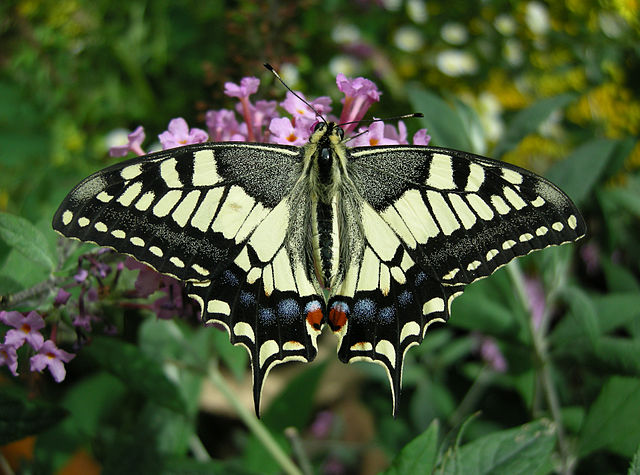
\includegraphics[height=1.5in]{butterfly.jpg}~
 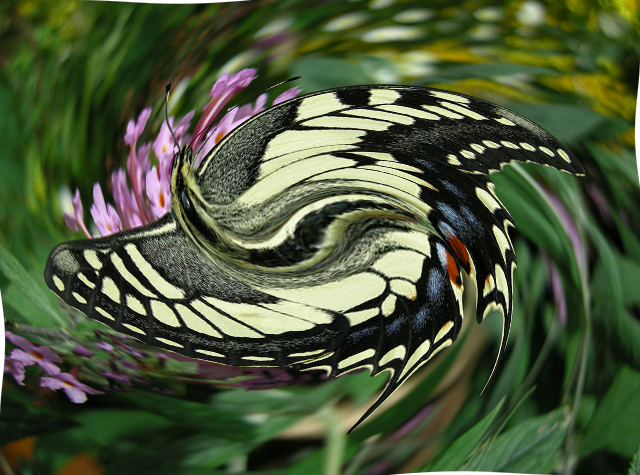
\includegraphics[height=1.5in]{swirledbutterfly.jpg}    
 %\caption{An example of a non-linear transformation.}\label{fig:swirl}
 \end{center}
%\end{image}

Many familiar transformations, such as rotations, reflections and shears, are linear. Every pixel $(x, y)$ of a digital image is treated as a vector $\begin{bmatrix}
x\\
y
\end{bmatrix}$.  To perform a linear transformation, we multiply the vector by a matrix.  The figure below shows the result of a linear transformation applied to the photo of a building.  Linear transformations keep the origin fixed, and map lines to lines. (See Practice Problem \ref{prob:linestolines})  ({\color{red} reference})

%\begin{figure}[h]
    \begin{center}
         
\includegraphics[height=1.5in]{building1.jpg}
~~~~~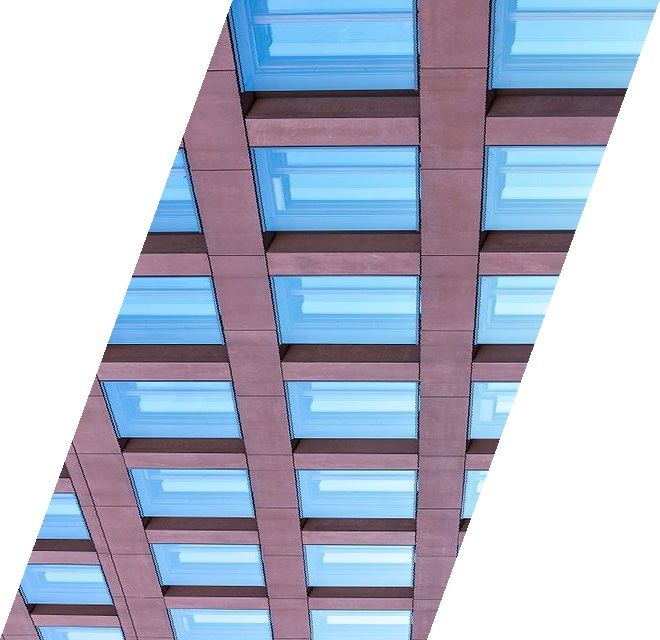
\includegraphics[height=1.5in]{building2.jpg}
      \end{center}
 %   \caption{An example of a linear transformation.}\label{fig:building}
%\end{figure}

\section*{Special Transformations of the Plane}
We now consider several basic linear transformations and the standard matrices associated with them.  The key concept is that if we want to understand what a linear transformation does, it is enough to understand what it does to basis vectors, such as standard basis vectors $\vec{i}$ and $\vec{j}$.  Caution: we can get into trouble if we try to construct a standard matrix for a non-linear transformation by tracking images of $\vec{i}$ and $\vec{j}$, as you will see in one of the Practice Problems!  %However, the examples in this section are all linear transformations. 

\subsection*{Horizontal and Vertical Scaling} 

% \begin{initprob} We will attempt to find the standard matrix $M$ of a linear transformation $T$ that stretches the image in Figure \ref{fig:vstretch} vertically by a factor of 2.  The difficulty here is that we are not sure at this point whether this kind of transformation is linear.  So, what we will do is construct a candidate for the standard matrix, and then test it to see whether it accomplishes the stretch.

\begin{initprob} Let us attempt to find the standard matrix $M$ of a transformation $T$ that stretches the image in Figure \ref{fig:vstretch} vertically by a factor of 2.  Assuming that this transformation is linear, we need to find what the transformation does to the standard basis vectors.  Once we have a candidate for the standard matrix, we will test it to make sure it accomplishes the stretch.

%\begin{figure}[h]
\begin{center}     
		\begin{tikzpicture}[scale=2]
\node[inner sep=0pt, anchor=base] (gulls) at (6.25mm,0)
  {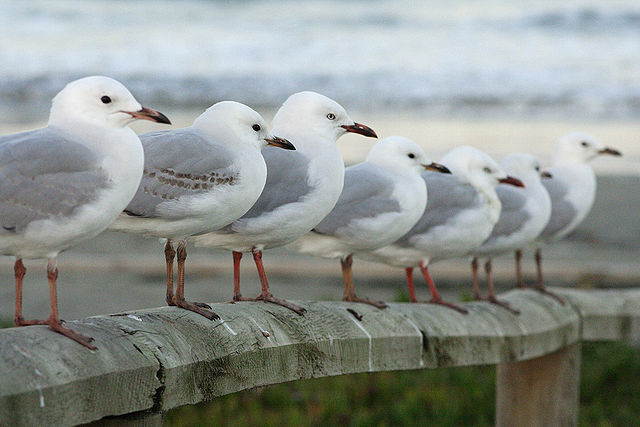
\includegraphics[width=25mm]{gulls.jpg}};
  \draw[<->] (-0.5,0)--(2,0);
  \draw[<->] (0,-0.5)--(0,2);
       \end{tikzpicture}
  \quad\quad
   \begin{tikzpicture}[scale=2]
 \node[inner sep=0pt, anchor=base]  (stretchedgulls) at (6.25mm,0)
  {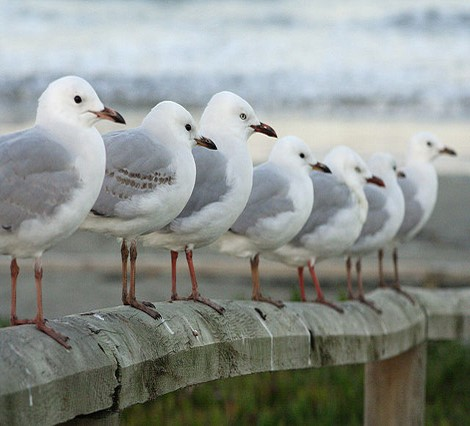
\includegraphics[width=25mm]{stretchedgulls.jpg}};
\draw[<->] (-0.5,0)--(2,0);
  \draw[<->] (0,-0.5)--(0,2);
    \end{tikzpicture}
\end{center}
%\caption{The original photo of seagulls was stretched vertically by a factor of 2.}
  \label{fig:vstretch} 
%\end{figure}


%\begin{figure}[h]
\begin{center}
\begin{tikzpicture}[scale=1.5]

  \draw[<->] (-0.5,0)--(2.5,0);
  \draw[<->] (0,-0.5)--(0,2.5);
   \draw[->,line width=1pt,red,-stealth](0,0)node[above=3mm, right=4mm]{$\vec{i}$}--(1,0);
    \draw[->,line width=1pt,blue,-stealth](0,0)node[above=6mm, left=0mm]{$\vec{j}$}--(0,1);
  \end{tikzpicture}
  \quad\quad
    \begin{tikzpicture}[scale=1.5]

\draw[<->] (-0.5,0)--(2.5,0);
  \draw[<->] (0,-0.5)--(0,2.5);
   \draw[->,line width=1pt,red,-stealth](0,0)node[above=3mm, right=3mm]{$T(\vec{i})$}--(1,0);
    \draw[->,line width=1pt,blue,-stealth](0,0)node[above=12mm, left=0mm]{$T(\vec{j})$}--(0,2);
    
 \end{tikzpicture}
\end{center}
%\caption{Images of $\vec{i}$ and $\vec{j}$ under a vertical stretch.}
  \label{fig:vstretchvectors} 
%\end{figure}
Consider what this transformation does to the standard unit vectors (see Figure \ref{fig:vstretchvectors}).  We observe that $T(\vec{i})=\vec{i}$ and $T(\vec{j})=2\vec{j}$.  This allows us to construct a candidate for the standard matrix $M$, by making the images of $\vec{i}$ and $\vec{j}$ the columns of $M$.  Thus, 
$$M=\begin{bmatrix}
1 & 0\\
0 & 2
\end{bmatrix}$$

We can now check to see what this matrix does to an arbitrary point $(a, b)$.  Treating this point as a vector $\begin{bmatrix}a\\b\end{bmatrix}$, we compute
$$M=\begin{bmatrix}
1 & 0\\
0 & 2
\end{bmatrix}\begin{bmatrix}a\\b\end{bmatrix}=\begin{bmatrix}a\\2b\end{bmatrix}$$
 Thus, this transformation takes point $(a, b)$ to point $(a, 2b)$.  So, the proposed transformation doubles all $y$-coordinates resulting in a vertical stretch by a factor of 2.
\end{initprob}






\begin{general} A vertical stretch (or compression) leaves $\vec{i}$ unchanged, and scales the vector $\vec{j}$ while preserving its vertical direction.  Thus, a vertical stretch (or compression) maps $\vec{i}$ to $\vec{i}$, and maps $\vec{j}$ to $k\vec{j}$ for some positive number $k$.  Similarly, a horizontal stretch (or compression) maps $\vec{i}$ to $k\vec{i}$, and maps $\vec{j}$ to $\vec{j}$.
\end{general}

\begin{formula}[Horizontal and Vertical Scaling] \label{form:horvertscaling}
  
 A linear transformation that scales objects in the plane vertically by a factor of $k$ is induced by 
  \begin{equation} \label{vscale}
M_v=\begin{bmatrix}
1 & 0\\
0 & k
\end{bmatrix}
\end{equation}
A linear transformation that scales objects in the plane horizontally by a factor of $k$ is induced by 
  \begin{equation} \label{hscale}
M_h=\begin{bmatrix}
k & 0\\
0 & 1
\end{bmatrix}
\end{equation}
where $k>0$.
\end{formula}

If we were to allow $k$ to be zero, what would the resulting transformations accomplish?  In what way would the resulting matrices be fundamentally different from matrices $M_v$ and $M_h$? (See Practice Problem \ref{prob:k0})  What would happen if $k$ were allowed to be negative?

\subsection*{Horizontal and Vertical Shears}
A \dfn{horizontal shear} is a transformation that takes an arbitrary point $(a, b)$ and maps it to the point $(a+kb, b)$.  The effect of this transformation is that all points along a fixed horizontal line slide to the left or to the right by a fixed amount.  Note that the higher the point $(a, b)$ is above the $x$-axis, the greater is the magnitude of $kb$, resulting in a greater amount of horizontal slide.

%\begin{figure}[h]
\begin{center}
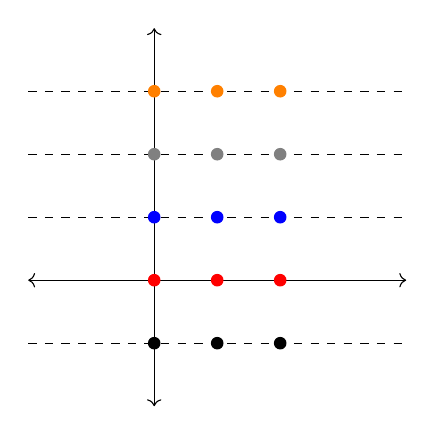
\begin{tikzpicture}[scale=0.8]

  \draw[<->] (-2,0)--(4,0);
   \draw[<->] (0,-2)--(0,4);
  \draw[dashed] (-2,-1)--(4,-1);
  \draw[dashed] (-2,1)--(4,1);
  \draw[dashed] (-2,2)--(4,2);
  \draw[dashed] (-2,3)--(4,3);
  
  
  \fill[] (0,-1) circle (0.1cm);
  \fill[] (1,-1) circle (0.1cm);
  \fill[] (2,-1) circle (0.1cm);
   
  \fill[red] (0,0) circle (0.1cm);
  \fill[red] (1,0) circle (0.1cm);
  \fill[red] (2,0) circle (0.1cm);
  
  \fill[blue] (0,1) circle (0.1cm);
  \fill[blue] (1,1) circle (0.1cm);
  \fill[blue] (2,1) circle (0.1cm);
  
  \fill[gray] (0,2) circle (0.1cm);
  \fill[gray] (1,2) circle (0.1cm);
  \fill[gray] (2,2) circle (0.1cm);
  
  \fill[orange] (0,3) circle (0.1cm);
  \fill[orange] (1,3) circle (0.1cm);
  \fill[orange] (2,3) circle (0.1cm);
  
   
  \end{tikzpicture}
   \quad\quad
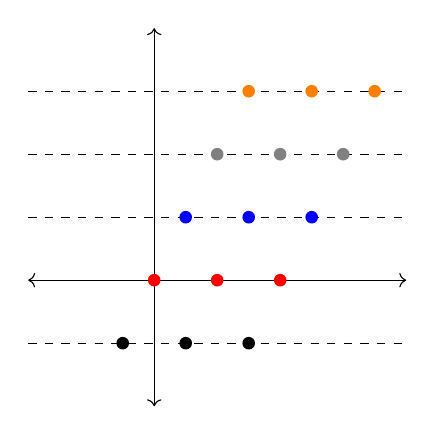
\begin{tikzpicture}[scale=0.8]

\draw[<->] (-2,0)--(4,0);
  \draw[<->] (0,-2)--(0,4);
  \draw[dashed] (-2,-1)--(4,-1);
  \draw[dashed] (-2,1)--(4,1);
  \draw[dashed] (-2,2)--(4,2);
  \draw[dashed] (-2,3)--(4,3);
   
   \fill[] (0-0.5,-1) circle (0.1cm);
  \fill[] (1-0.5,-1) circle (0.1cm);
  \fill[] (2-0.5,-1) circle (0.1cm);
   
  \fill[red] (0,0) circle (0.1cm);
  \fill[red] (1,0) circle (0.1cm);
  \fill[red] (2,0) circle (0.1cm);
  
  \fill[blue] (0+0.5,1) circle (0.1cm);
  \fill[blue] (1+0.5,1) circle (0.1cm);
  \fill[blue] (2+0.5,1) circle (0.1cm);
  
  \fill[gray] (0+1,2) circle (0.1cm);
  \fill[gray] (2,2) circle (0.1cm);
  \fill[gray] (3,2) circle (0.1cm);
  
  \fill[orange] (1.5,3) circle (0.1cm);
  \fill[orange] (2.5,3) circle (0.1cm);
  \fill[orange] (3.5,3) circle (0.1cm);
 
 \end{tikzpicture}
\end{center}
%\caption{The action of a horizontal shear transformation $(k>0)$ on a sample of points in $\RR^2$.}
  \label{fig:verticalshearex} 
%\end{figure}

Adding a scalar multiple of the $y$ component to the $x$ component can be accomplished by a matrix transformation.  Observe that 
$$\begin{bmatrix}
1 & k\\
0 & 1
\end{bmatrix}\begin{bmatrix}a\\b\end{bmatrix}=\begin{bmatrix}a+kb\\b\end{bmatrix}$$

A \dfn{vertical shear} is a transformation that takes an arbitrary point $(a, b)$ and maps it to the point $(a, b+ka)$.  This too, is a matrix transformation.
$$\begin{bmatrix}
1 & 0\\
k & 1
\end{bmatrix}\begin{bmatrix}a\\b\end{bmatrix}=\begin{bmatrix}a\\b+ka\end{bmatrix}$$


\begin{formula}[Horizontal and Vertical Shears]\label{form:shears}
  
A linear transformation that shears the plane horizontally is induced by 
  \begin{equation} 
M_{hs}=\begin{bmatrix}
1 & k\\
0 & 1
\end{bmatrix}
\end{equation}
A linear transformation that shears the plane vertically is induced by
  \begin{equation} 
M_{vs}=\begin{bmatrix}
1 & 0\\
k & 1
\end{bmatrix}
\end{equation}
\end{formula}

\begin{example} Find the standard matrix $M_{vs}$ of a linear transformation $T$ that {\it shears} the image of a seagull as shown in the figure below. %\ref{fig:vshears}. 

%\begin{figure}[h]
\begin{center}
   
		\begin{tikzpicture}[scale=2]
\node[inner sep=0pt, anchor=base] (gulls) at (6.25mm,0)
  {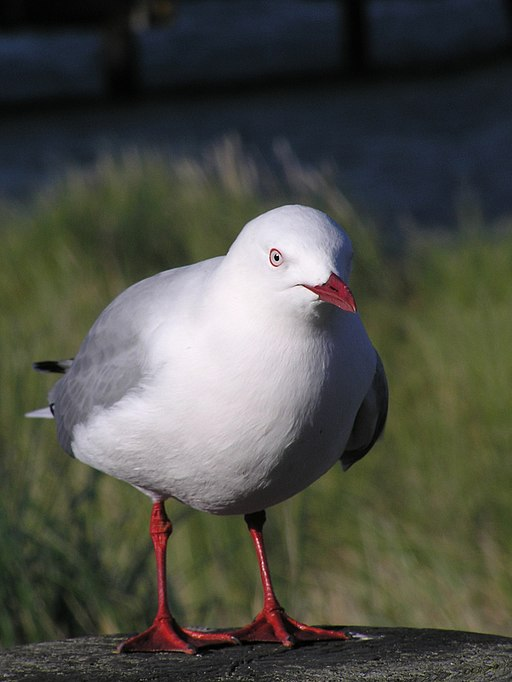
\includegraphics[width=25mm]{gull.jpg}};
  \draw[<->] (-0.5,0)--(2,0);
  \draw[<->] (0,-0.5)--(0,2);
       \end{tikzpicture}
  \quad\quad
\begin{tikzpicture}[scale=2]
 \node[inner sep=0pt, anchor=base]  (stretchedgulls) at (6.25mm,0)
  {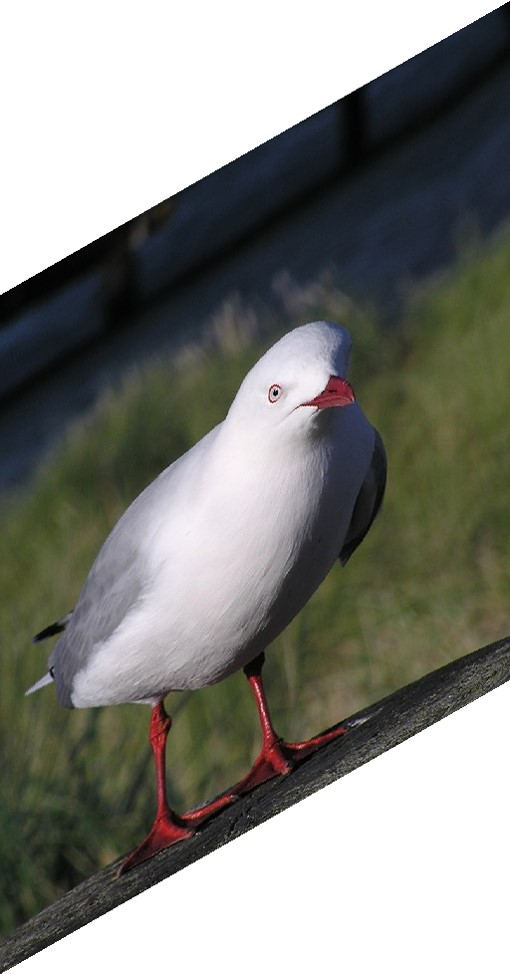
\includegraphics[width=25mm]{shearedgull.jpg}};
  
  \draw (0.5,0)node[above=3mm, right=0mm]{$30^{\circ}$} arc (0:30:0.5) ;

\draw[<->] (-0.5,0)--(2,0);
  \draw[<->] (0,-0.5)--(0,2);
    
 \end{tikzpicture}
\end{center}
%\caption{The original photo was sheared vertically.}
  \label{fig:vshears} 
%\end{figure}

\begin{explanation}
Consider what this transformation does to the standard unit vectors. %(See Figure \ref{fig:verticalshearex})

%\begin{figure}[h]
\begin{center}

\begin{tikzpicture}[scale=2]

  \draw[<->] (-0.5,0)--(1.5,0);
  \draw[<->] (0,-0.5)--(0,1.5);
   \draw[->,line width=1pt,red,-stealth](0,0)node[above=3mm, right=6mm]{$\vec{i}$}--(1,0);
    \draw[->,line width=1pt,blue,-stealth](0,0)node[above=8mm, left=0mm]{$\vec{j}$}--(0,1);
  \end{tikzpicture}
   \quad\quad
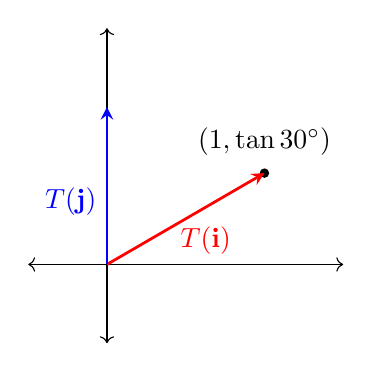
\begin{tikzpicture}[scale=2]

\draw[<->] (-0.5,0)--(1.5,0);
  \draw[<->] (0,-0.5)--(0,1.5);
  \fill[] (1,0.58)node[above=1mm]{$(1,\tan 30^{\circ})$} circle (0.03cm);   
   \draw[->,line width=1pt,red,-stealth](0,0)node[above=3mm, right=8mm]{$T(\vec{i})$}--(1,0.58);
    \draw[->,line width=1pt,blue,-stealth](0,0)node[above=8mm, left=0mm]{$T(\vec{j})$}--(0,1);
  \end{tikzpicture}
  \end{center}
%\caption{The action of a vertical shear transformation on the standard unit vectors.}
  \label{fig:verticalshearex} 
%\end{figure}

The tip of the vector $\vec{i}$ slides up a vertical line and its $x$-component remains the same.  Vector $\vec{j}$ stays fixed.  We observe that $T(\vec{i})=\begin{bmatrix}
1 \\
\tan 30^{\circ}
\end{bmatrix}=\begin{bmatrix}
1 \\
\sqrt{3}/3
\end{bmatrix}$ and $T(\vec{j})=\vec{j}$.  This allows us to construct $M_{vs}$, by making the images of $\vec{i}$ and $\vec{j}$ the columns of $M_{vs}$.  Thus, 
$$M_{vs}=\begin{bmatrix}
1 & 0\\
\sqrt{3}/3 & 1
\end{bmatrix}$$
\end{explanation}
\end{example}

%\begin{figure}[h]
%\centering


%\begin{tikzpicture}[scale=2]

%\draw[<->] (-0.5,0)--(1.5,0);
 % \draw[<->] (0,-0.5)--(0,1.5);
 % \fill[] (1,0.58)node[above=1mm,right=1mm]{$(1,\tan \alpha)$} circle (0.03cm);   
  % \draw[->,line width=1pt,red,-stealth](0,0)node[above=10mm, right=4mm]{$T(\vec{i})$}--(1,0.58);
   % \draw[->,line width=1pt,blue,-stealth](0,0)node[above=8mm, left=0mm]{$T(\vec{j})$}--(0,1);
    %\draw (0.5,0)node[above=3mm, right=0mm]{$\alpha$} arc (0:30:0.5) ;
 
 %\end{tikzpicture}
%\quad\quad
%\begin{tikzpicture}[scale=2]

%\draw[<->] (-0.5,0)--(1.5,0);
 % \draw[<->] (0,-0.5)--(0,1.5);
 % \fill[] (0.58,1)node[above=1mm,right=1mm]{$(\tan \beta ,1)$} circle (0.03cm);   
  % \draw[->,line width=1pt,red,-stealth](0,0)node[below=3mm, right=6mm]{$T(\vec{i})$}--(1,0);
   % \draw[->,line width=1pt,blue,-stealth](0,0)node[above=8mm,right=6mm]{$T(\vec{j})$}--(0.58,1);
 %\draw (0.25,0.43)node[above=4mm, left=0mm]{$\beta$} arc (60:90:0.5) ;
 %\end{tikzpicture}

%\caption{Graphical illustration of non-commutativity of matrix multiplication.}
 % \label{fig:verthorshears} 
%\end{figure}



%\begin{general} There are vertical and horizontal shears.  Figure \ref{fig:shear} shows the effect of shears on vectors $\vec{i}$ and $\vec{j}$.
%\end{general}



%A vertical shear leaves $\vec{j}$ fixed and maps $\vec{i}$ to $\begin{bmatrix}1\\\tan\alpha\end{bmatrix}$.  A horizontal shear fixes $\vec{i}$ and maps $\vec{j}$ to $\begin{bmatrix}\tan\beta\\1\end{bmatrix}$.  If we treat $\tan\alpha$ and $\tan\beta$ as simple constants, we get the following matrices that induce shears.



\subsection*{Rotations about the Origin}
Recall that to prove that a transformation $T$ is linear, we have to show that for all vectors $\vec{u}$ and $\vec{v}$ and scalars $k_1$ and $k_2$ we have
\begin{equation}\label{eq:rotlintrans}
T(k_1\vec{u}+k_2\vec{v})=k_1 T(\vec{u})+k_2 T(\vec{v})
\end{equation}

We are used to going through this verification algebraically.  In some situations, however, it is instructive to think about this property geometrically.  Consider a transformation $R_{\theta}$ that rotates every point in the plane counter-clockwise through angle $\theta$ about the origin.  Is $R_{\theta}$ a linear transformation?

Figure \ref{fig:rotlintransleft} illustrates the left-hand side of Equation \ref{eq:rotlintrans}.  Scalar multiples of $\vec{u}$ and $\vec{v}$ are added in the domain, then the sum is rotated through angle $\theta$ by $R_{\theta}$.

%\begin{figure}[h]
\begin{center}

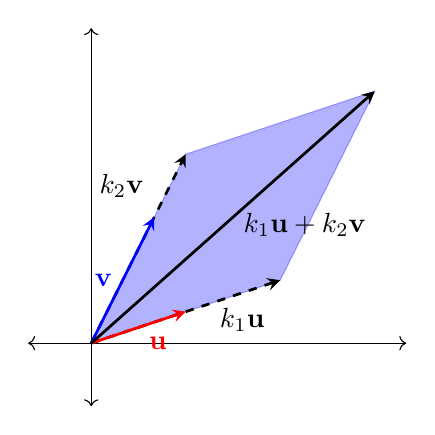
\begin{tikzpicture}[scale=0.8]

  \draw[<->] (-1,0)--(5,0);
  \draw[<->] (0,-1)--(0,5);
  \filldraw[blue, opacity=0.3](0,0)--(3,1)--(4.5,4)--(1.5,3)--cycle;
  \draw[->,line width=1pt,-stealth, dashed](0,0)node[above=3mm, right=15mm]{$k_1\vec{u}$}--(3,1);
   \draw[->,line width=1pt,red,-stealth](0,0)node[above=0mm, right=6mm]{$\vec{u}$}--(1.5,0.5);
   \draw[->,line width=1pt,-stealth, dashed](0,0)node[above=20mm, left=-8mm]{$k_2\vec{v}$}--(1.5,3);
    \draw[->,line width=1pt,blue,-stealth](0,0)node[above=8mm, left=-4mm]{$\vec{v}$}--(1,2);
    \draw[->,line width=1pt,-stealth](0,0)node[above=15mm, right=18mm]{$k_1\vec{u}+k_2\vec{v}$}--(4.5,4);
  \end{tikzpicture}
   \quad
\begin{tikzpicture}[scale=0.8]
\draw[->,line width=1pt,-stealth](0,0)node[above=15mm, left=18mm]{$R_{\theta}(k_1\vec{u}+k_2\vec{v})$}--(-4,4.5);
\draw[<->] (-5,0)--(1,0);
  \draw[<->] (0,-1)--(0,5);
  
  \end{tikzpicture}
  \end{center}
%\caption{Vectors $k_1\vec{u}$ and $k_2\vec{v}$ are added in the domain, then $R_{\theta}$ is applied to the sum.}
  \label{fig:rotlintransleft} 
%\end{figure}

The above figure  illustrates the right-hand side of Equation \ref{eq:rotlintrans}.  First, vectors $\vec{u}$ and $\vec{v}$ are rotated through angle $\theta$, then their images are scaled and added together.  Because the diagonal of a parallelogram rotates with the parallelogram, it is clear that 
$$R_{\theta}(k_1\vec{u}+k_2\vec{v})=k_1R_{\theta}(\vec{u})+k_2R_{\theta}(\vec{v})$$
So, intuition tells us that $R_{\theta}$ is linear.



%\begin{figure}[h]

\begin{image}[4.5in]\label{fig:rotlintransright} 
\begin{tikzpicture}[scale=0.8]

  \draw[<->] (-1,0)--(5,0);
  \draw[<->] (0,-1)--(0,5);
  
  
   \draw[->,line width=1pt,red,-stealth](0,0)node[above=0mm, right=6mm]{$\vec{u}$}--(1.5,0.5);
  
    \draw[->,line width=1pt,blue,-stealth](0,0)node[above=8mm, left=-4mm]{$\vec{v}$}--(1,2);
   
  \end{tikzpicture}
   \quad
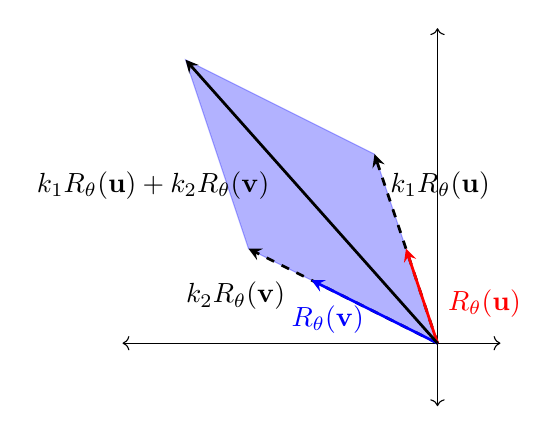
\begin{tikzpicture}[scale=0.8]
\draw[<->] (-5,0)--(1,0);
  \draw[<->] (0,-1)--(0,5);
  \filldraw[blue, opacity=0.3](0,0)--(-1,3)--(-4,4.5)--(-3,1.5)--cycle;
  \draw[->,line width=1pt,-stealth, dashed](0,0)node[above=6mm, left=18mm]{$k_2R_{\theta}(\vec{v})$}--(-1,3);
   \draw[->,line width=1pt,red,-stealth](0,0)node[above=5mm, right=0mm]{$R_{\theta}(\vec{u})$}--(-0.5,1.5);
   \draw[->,line width=1pt,-stealth, dashed](0,0)node[above=20mm, left=-8mm]{$k_1R_{\theta}(\vec{u})$}--(-3,1.5);
    \draw[->,line width=1pt,blue,-stealth](0,0)node[above=3mm, left=8mm]{$R_{\theta}(\vec{v})$}--(-2,1);
    \draw[->,line width=1pt,-stealth](0,0)node[above=20mm, left=20mm]{$k_1R_{\theta}(\vec{u})+k_2R_{\theta}(\vec{v})$}--(-4,4.5);
  
  \end{tikzpicture}
  \end{image}
 
%\caption{Vectors $\vec{u}$ and $\vec{v}$ are rotated individually, then scalar multiples of their images, $k_1R_{\theta}(\vec{u})$ and $k_2R_{\theta}(\vec{v})$, are added together.}
  
%\end{figure}

Before we consider the general standard matrix of $R_{\theta}$, let's take a look at a specific example.

\begin{example} Find the standard matrix $M_{\theta}$ of a linear transformation $R_{\theta}$ that rotates the image  by $45^{\circ}$ counterclockwise.


%\begin{figure}[h]
\begin{center}
\begin{image}
    
		\begin{tikzpicture}[scale=1.3]
\node[inner sep=0pt] (tower) at (0,0)
  {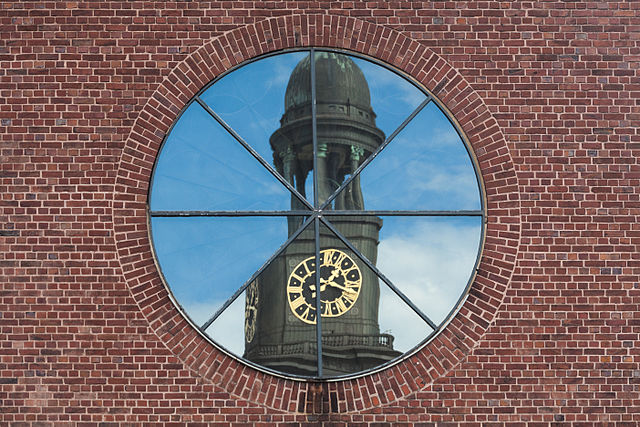
\includegraphics[width=45mm]{tower.jpg}};
  \draw[<->] (-2,0)--(2,0);
  \draw[<->] (0,-2)--(0,2);
       \end{tikzpicture}
\begin{tikzpicture}[scale=1.3]
\node[inner sep=0pt] (tower) at (0,0)
  {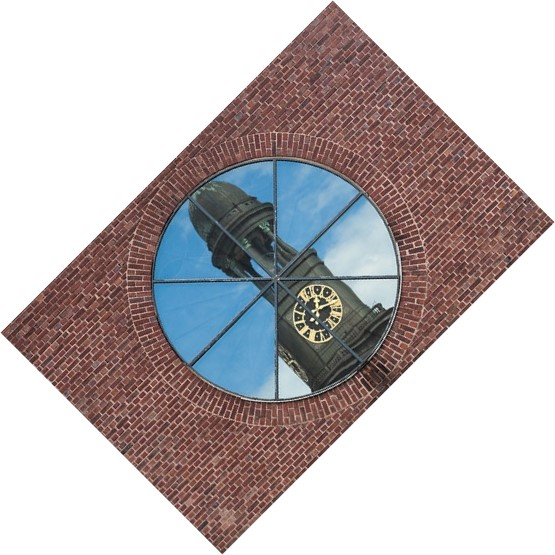
\includegraphics[width=50mm]{rotatedtower.jpg}};
  \draw[<->] (-2,0)--(2,0);
  \draw[<->] (0,-2)--(0,2);
       \end{tikzpicture}
\end{image}
\end{center}
%\caption{The original photo was rotated about the origin.}
  \label{fig:rotationofpic} 
%\end{figure}

\begin{explanation}  Consider the action of $R_{\theta}$ on the standard unit vectors. %(See Figure \ref{fig:rotationex})

%\begin{figure}[h]
\begin{center}
\begin{image}     
\begin{tikzpicture}[scale=3]

  \draw[<->] (-0.5,0)--(1.5,0);
  \draw[<->] (0,-0.5)--(0,1.5);
   \draw[->,line width=1pt,red,-stealth](0,0)node[above=3mm, right=6mm]{$\vec{i}$}--(1,0);
    \draw[->,line width=1pt,blue,-stealth](0,0)node[above=8mm, left=0mm]{$\vec{j}$}--(0,1);
  \end{tikzpicture}
  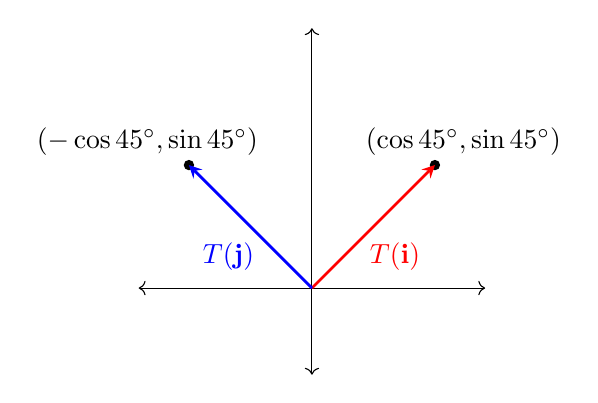
\begin{tikzpicture}[scale=2.2]

\draw[<->] (-1,0)--(1,0);
  \draw[<->] (0,-0.5)--(0,1.5);
  \fill[] (0.71,0.71)node[above=3mm, right=-10mm]{$(\cos 45^{\circ},\sin 45^{\circ})$} circle (0.03cm); 
  \fill[] (-0.71,0.71)node[above=3mm,left=-10mm]{$(-\cos 45^{\circ}, \sin 45^{\circ})$} circle (0.03cm); 
   \draw[->,line width=1pt,red,-stealth](0,0)node[above=4mm, right=6mm]{$T(\vec{i})$}--(0.71,0.71);
    \draw[->,line width=1pt,blue,-stealth](0,0)node[above=4mm, left=6mm]{$T(\vec{j})$}--(-0.71,0.71);
 
 \end{tikzpicture}
 \end{image}
\end{center}
%\caption{The action of $R_{\theta}$ on the standard unit vectors.}
  \label{fig:rotationex} 
%\end{figure}


We observe that $R_{\theta}(\vec{i})=\begin{bmatrix}
\cos 45^{\circ} \\
\sin 45^{\circ}
\end{bmatrix}=\begin{bmatrix}
\frac{\sqrt{2}}{2} \\
\frac{\sqrt{2}}{2}
\end{bmatrix}$ and $R_{\theta}(\vec{j})=\begin{bmatrix}
-\sin 45^{\circ} \\
\cos 45^{\circ}
\end{bmatrix}=\begin{bmatrix}
-\frac{\sqrt{2}}{2} \\
\frac{\sqrt{2}}{2}
\end{bmatrix}$.  This allows us to construct the matrix $M_{\theta}$, by making the images of $\vec{i}$ and $\vec{j}$ the columns of $M_{\theta}$.  Thus, 
$$M_{\theta}=\begin{bmatrix}
\frac{\sqrt{2}}{2} & -\frac{\sqrt{2}}{2}\\
\frac{\sqrt{2}}{2} & \frac{\sqrt{2}}{2}
\end{bmatrix}$$
\end{explanation}
\end{example}

\begin{general} We find the standard rotation matrix by determining the images of vectors $\vec{i}$ and $\vec{j}$.
\end{general}


%\begin{figure}[h]
\begin{center}
\begin{tikzpicture}[scale=2.5]
  \draw[<->] (-0.5,0)--(1.5,0);
  \draw[<->] (0,-0.5)--(0,1.5);
   \draw[->,line width=1pt,red,-stealth](0,0)node[above=3mm, right=6mm]{$\vec{i}$}--(1,0);
    \draw[->,line width=1pt,blue,-stealth](0,0)node[above=8mm, left=0mm]{$\vec{j}$}--(0,1);
  \end{tikzpicture}
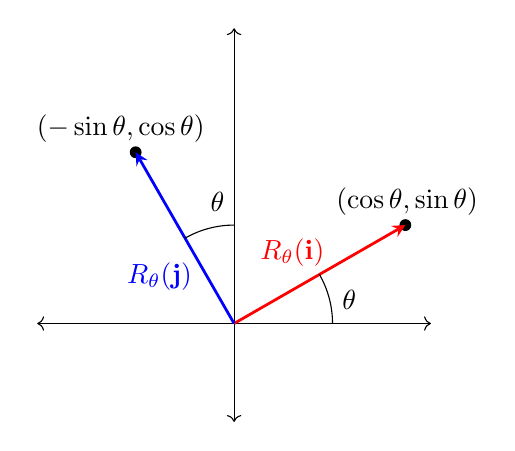
\begin{tikzpicture}[scale=2.5]
\draw[<->] (-1,0)--(1,0);
  \draw[<->] (0,-0.5)--(0,1.5);
  \fill[] (0.87,0.5)node[above=3mm, right=-10mm]{$(\cos \theta,\sin \theta)$} circle (0.03cm); 
  \fill[] (-0.5, 0.87)node[above=3mm,left=-10mm]{$(-\sin \theta, \cos \theta)$} circle (0.03cm); 
   \draw[->,line width=1pt,red,-stealth](0,0)node[above=9mm, right=2mm]{$R_{\theta}(\vec{i})$}--(0.87,0.5);
    \draw[->,line width=1pt,blue,-stealth](0,0)node[above=6mm, left=4mm]{$R_{\theta}(\vec{j})$}--(-0.5, 0.87);
 \draw (0.5,0)node[above=3mm, right=0mm]{$\theta$} arc (0:30:0.5) ;
  \draw (0,0.5)node[above=3mm, left=0mm]{$\theta$} arc (90:120:0.5) ;
 \end{tikzpicture}
\end{center}
%\caption{Images of $\vec{i}$ and $\vec{j}$ under a counter-clockwise rotation about the origin.}
 % \label{fig:rotationij} 
%\end{figure}

\begin{formula}[Counterclockwise Rotation]
  
  A linear transformation that rotates the plane counterclockwise through angle $\theta$ about the origin is induced by
\begin{equation} \label{eq:rotation}
M_{\theta}=\begin{bmatrix}
\cos\theta & -\sin\theta\\
\sin\theta & \cos\theta
\end{bmatrix}
\end{equation}
\end{formula}

\subsection*{Reflections about Lines of the Form $y=mx$}
When a point is reflected about a line, its image is located on the opposite side of the line and the same distance away from the line as the original point.

For example, Figure \ref{fig:reflectdefinition} shows the reflection of point $A$ about line $l$.  Note that the reflection lies on a line through $A$ perpendicular to $l$.

%\begin{figure}[h]
\begin{center}   
\begin{tikzpicture}[scale=1.2]

   \draw[line width=1pt](-1,2)node[below=2mm, left=1mm]{$l$}--(1,-2);
  \draw[thin, dashed](-2,-1.5)node[below=2mm]{}--(2,0.5);
  
  \fill[red](1,0) circle (0.08)node[above=4mm, right=-1mm]{$A$};
  \fill[](-0.6,-0.8) circle (0.08)node[above=5mm, left=-2mm]{};
    \end{tikzpicture}
    \end{center}
  % \caption{Reflection of point $A$ about line $l$.}
   %     \label{fig:reflectdefinition}
    %\end{figure}
    
    Arguing in a manner similar to our discussion of linearity of rotations, we can see that reflections are also linear.  Our task is to find the matrix of a reflection of the plane about an arbitrary line through the origin.
  
  We will start by finding reflections about the axes.  You can easily do this on your own by finding the images of vectors $\vec{i}$ and $\vec{j}$.  
  
  We will start with the reflection about the $x$-axis.
  
  $$\vec{i}=\begin{bmatrix}1\\0\end{bmatrix}\quad\text{maps to}\quad\begin{bmatrix}\answer{1}\\\answer{0}\end{bmatrix}$$
  
  $$\vec{j}=\begin{bmatrix}0\\1\end{bmatrix}\quad\text{maps to}\quad\begin{bmatrix}\answer{0}\\\answer{-1}\end{bmatrix}$$
  
  So, the standard matrix that induces the reflection about the $x$-axis is
  $$\begin{bmatrix}\answer{1}&\answer{0}\\\answer{0}&\answer{-1}\end{bmatrix}$$
Next, we will consider the reflection about the $y$-axis.
$$\vec{i}=\begin{bmatrix}1\\0\end{bmatrix}\quad\text{maps to}\quad\begin{bmatrix}\answer{-1}\\\answer{0}\end{bmatrix}$$
  
  $$\vec{j}=\begin{bmatrix}0\\1\end{bmatrix}\quad\text{maps to}\quad\begin{bmatrix}\answer{0}\\\answer{1}\end{bmatrix}$$
  
  Thus, the standard matrix that induces the reflection about the $y$-axis is
  $$\begin{bmatrix}\answer{-1}&\answer{0}\\\answer{0}&\answer{1}\end{bmatrix}$$
  
  Now we will turn our attention to transformations that reflect the plane about the line $y=mx$.  We will assume that $m\neq 0$.
  
  Consider the vector $\vec{i}$ and its reflection. (See Figure \ref{fig:t1})
%\begin{figure}[h]
\begin{center}  
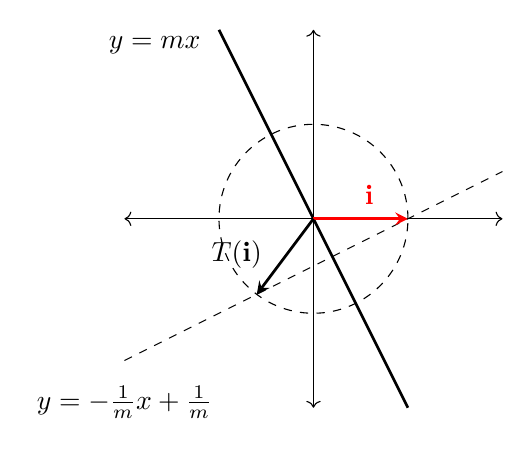
\begin{tikzpicture}[scale=1.2]

  \draw[<->] (-2,0)--(2,0);
  \draw[<->] (0,-2)--(0,2);

  \draw[line width=1pt](-1,2)node[below=2mm, left=1mm]{$y=mx$}--(1,-2);
  \draw[thin, dashed](-2,-1.5)node[below=2mm]{$y=-\frac{1}{m}x+\frac{1}{m}$}--(2,0.5);
  
  \draw[->,line width=1pt, -stealth, red](0,0)--(1,0)node[above=3mm, left=3mm]{$\vec{i}$};
  \draw[->,line width=1pt, -stealth](0,0)--(-0.6,-0.8)node[above=5mm, left=-2mm]{$T(\vec{i})$};
  \draw[dashed] (0,0) circle (1);
 
  \end{tikzpicture}
  \end{center}
%   \caption{Image of $\vec{i}$ under  $T$.}
 %       \label{fig:t1}
  %  \end{figure}
   
   
   
   Observe that the head of the image vector, $T(\vec{i})$, will lie on the line that passes through $(1,0)$ and is perpendicular to the line $y=mx$.  The equation of this line is given by
   
   \begin{equation}\label{eq:reflectionline} 
   y=-\frac{1}{m}x+\frac{1}{m}
   \end{equation}
   
 The head of $T(\vec{i})$ will also lie on the circle with equation
   $$x^2+y^2=1$$
   
   
   To find the image of $\vec{i}$ we need to determine where the line  $y=-\frac{1}{m}x+\frac{1}{m}$ intersects the circle.  Substitution gives us
   
   $$x^2+\left(-\frac{1}{m}x+\frac{1}{m}\right)^2=1$$
   After a little algebra we get
   $$\left(1+\frac{1}{m^2}\right)x^2-\left(\frac{2}{m^2}\right)x+\left(\frac{1}{m^2}-1\right)=0$$
   The quadratic formula yields 
   $$x=1\quad\text{and}\quad x=\frac{1-m^2}{m^2+1}$$
   
   The solution $x=1$ corresponds to the head of the vector $\vec{i}$.  So, the $x$-component of $T(\vec{i})$ is $x=\frac{1-m^2}{m^2+1}$.  We find the $y$-component of $T(\vec{i})$ by
   substituting $x=\frac{1-m^2}{m^2+1}$ into Equation \ref{eq:reflectionline}.
   $$ y=-\frac{1}{m}\left(\frac{1-m^2}{m^2+1}\right)+\frac{1}{m}=\frac{2m}{m^2+1}$$
   Thus, the image of $\vec{i}$ under this reflection is given by
   $$T(\vec{i})=\begin{bmatrix}\frac{1-m^2}{m^2+1}\\\frac{2m}{m^2+1}\end{bmatrix}$$
   
Next we need to find the image of $\vec{j}$. The head of $T(\vec{j})$ is located at one of the intersections of line $y=-\frac{1}{m}x+1$ and the circle $x^2+y^2=1$.  
   
%    \begin{figure}[h]
  \begin{center}
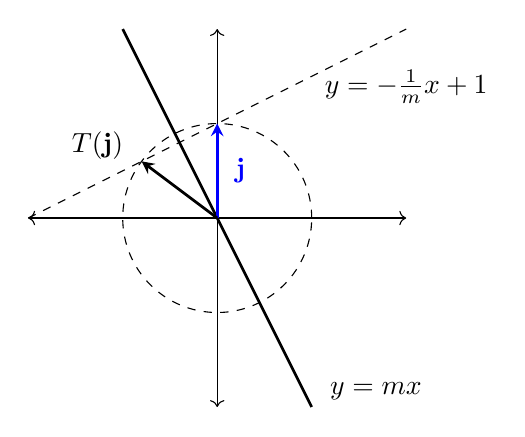
\begin{tikzpicture}[scale=1.2]

  \draw[<->] (-2,0)--(2,0);
  \draw[<->] (0,-2)--(0,2);
 
  \draw[line width=1pt](-1,2)--(1,-2)node[above=2mm, right=1mm]{$y=mx$};
  \draw[thin, dashed](-2,0)--(2,2)node[below=4mm]{$y=-\frac{1}{m}x+1$};
  
  \draw[->,line width=1pt, -stealth, blue](0,0)--(0,1)node[below=6mm, right=1mm]{$\vec{j}$};
  \draw[->,line width=1pt, -stealth](0,0)--(-0.8,0.6)node[above=2mm, left=1mm]{$T(\vec{j})$};
  \draw[dashed] (0,0) circle (1);
  \end{tikzpicture}
  \end{center}
%\caption{Image of $\vec{j}$ under $T$.}
 %       \label{fig:t2}
  %  \end{figure}

We leave it to the reader to verify that
\begin{equation}\label{eq:imageofj} T(\vec{j})=\begin{bmatrix}\frac{2m}{m^2+1}\\\frac{m^2-1}{m^2+1}\end{bmatrix}\end{equation}

The standard matrix of this reflection is then given by 
$$M_{y=mx}=\begin{bmatrix}\frac{1-m^2}{m^2+1} & \frac{2m}{m^2+1}\\\frac{2m}{m^2+1} & \frac{m^2-1}{m^2+1}\end{bmatrix}=\frac{1}{1+m^2}\begin{bmatrix}
1-m^2 & 2m \\
2m & m^2-1
\end{bmatrix}$$









\begin{formula}[Reflection about the line $y=mx$]
  
  A linear transformation that reflects the plane about the line $y=mx$ is induced by
\begin{equation} \label{eq:reflectionymx}
M_{y=mx}=\frac{1}{1+m^2}\begin{bmatrix}
1-m^2 & 2m \\
2m & m^2-1
\end{bmatrix}
\end{equation}
\end{formula}

\begin{example}\label{ex:reflectedduck} Find the standard matrix $M$ of a linear transformation that reflects the image in Figure \ref{fig:reflectedduck} about the line $y=\frac{3}{5}x$.

%\begin{figure}[h]
\begin{center}
		\begin{tikzpicture}[scale=2]
\node[inner sep=0pt, anchor=base] (gulls) at (6.25mm,0)
  {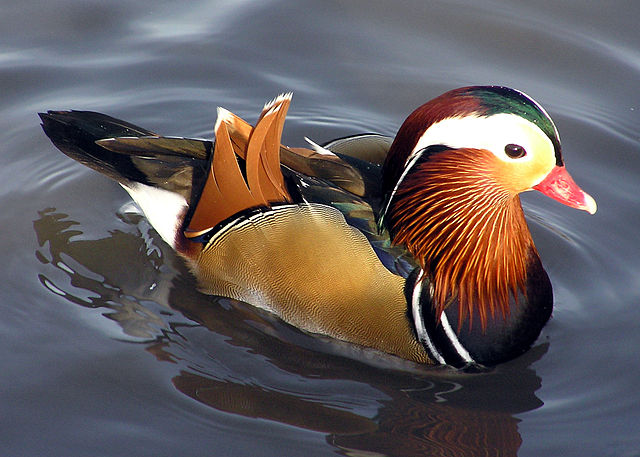
\includegraphics[width=25mm]{duck.jpg}};
  \draw[<->] (-0.5,0)--(2,0);
  \draw[<->] (0,-0.5)--(0,1.5);
  \draw[red,thick] (0,0)--(2,1.2)node[above=2mm, left=1mm]{$y=\frac{3}{5}x$};
       \end{tikzpicture}
   \quad\quad
\begin{tikzpicture}[scale=2]
 \node[inner sep=0pt, anchor=base]  (stretchedgulls) at (6.875mm,-4.2mm)
  {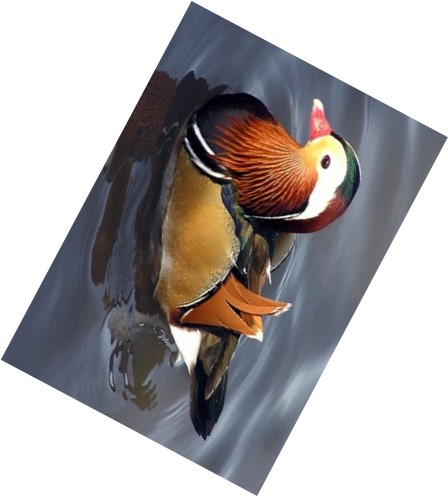
\includegraphics[width=27.5mm]{reflectedduck.jpg}};
  
\draw[red,thick] (0,0)--(2,1.2)node[above=2mm, left=1mm]{$y=\frac{3}{5}x$};
\draw[<->] (-0.5,0)--(2,0);
  \draw[<->] (0,-0.5)--(0,1.5);
    
 \end{tikzpicture}
 \end{center}
% \caption{The original photo of the duck was reflected about he line $y=\frac{3}{5}x$.}
%  \label{fig:reflectedduck} 
%\end{figure}
\begin{explanation}
$$M=\frac{1}{1+9/25}\begin{bmatrix}1-9/25 & 6/5\\6/5 & 9/25 -1\end{bmatrix}=\frac{25}{34}\begin{bmatrix}16/25 & 6/5\\6/5 & -16/25\end{bmatrix}=\begin{bmatrix}8/17 & 15/17\\15/17 & -8/17\end{bmatrix}$$
\end{explanation}
\end{example}

Note that the eye of the duck in Figure \ref{fig:reflectedduck} is located on the line $y=\frac{3}{5}x$.  The reflection leaves the eye fixed in place.  The eye is an example of a \dfn{fixed point}.  In Practice Problem \ref{prob:fixedpoint} {\color{red} reference} you will be asked to show that every point along the line $y=\frac{3}{5}x$ is a fixed point.

\subsection*{Composition of Linear Transformations}

If a linear transformation is followed by another linear transformation, the resulting transformation can be represented by a product of the two matrices that induce the individual transformations.  Thus, if $T_1$ is induced by $M_1$ and $T_2$ is induced by $M_2$, then $T=T_2\circ T_1$ is induced by $M=M_2M_1$.

\begin{center}
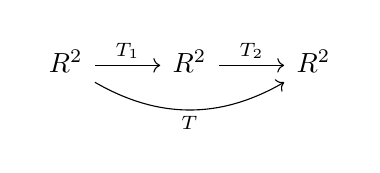
\begin{tikzpicture}
\node{
\begin{tikzcd}
\RR^2\rar{T_1}\arrow[black, bend right]{rr}[black,swap]{T}  & \RR^2 \rar{T_2}  & \RR^2
\end{tikzcd}
};
\end{tikzpicture}
\end{center}

Remember that matrix multiplication is not commutative, so the order in which the matrices are multiplied is of utmost importance.

\begin{initprob}\label{init:reflectioncomp}  In this problem we will consider compositions of two reflections and use geometry to illustrate non-commutativity of matrix multiplication.  
Let $$T_{y=-2x}:\RR^2\rightarrow \RR^2$$ be a reflection about the line $y=-2x$.  Let $$T_{y=x}:\RR^2\rightarrow \RR^2$$ be a reflection about the line $y=x$. We will denote the standard matrices for these transformations by $M_{y=-2x}$ and $M_{y=x}$, and
%$$M_{y=-2x}=\begin{bmatrix}
%-3/5 & -4/5 \\
%-4/5 & 3/5
%\end{bmatrix}\quad\text{and}\quad
%M_{y=x}=\begin{bmatrix}
%0 & 1 \\
%1 & 0
%\end{bmatrix}$$
 use geometry to demonstrate that $M_{y=x}M_{y=-2x}\neq M_{y=-2x}M_{y=x}$.  
 
 To do this, consider transformations $T_1=T_{y=x}\circ T_{y=-2x}$ and $T_2=T_{y=-2x}\circ T_{y=x}$.  Transformation $T_1$ is induced by $M_{y=x}M_{y=-2x}$, and $T_2$ is induced by $M_{y=-2x}M_{y=x}$.

Figure \ref{fig:reflectioncomp} illustrates the action of $T_1$ on a single point $A$.  First, $A$ is reflected about the line $y=-2x$, then $A$ is reflected about the line $y=x$.   

Figure \ref{fig:reflectioncomp} also shows the action of $T_2$ on the same point $A$.  The point is first reflected about the line $y=x$, followed by a reflection about the line $y=-2x$.  The final images of point $A$ under $T_1$ and $T_2$ are clearly different.

%\begin{figure}[h]
\begin{center}   
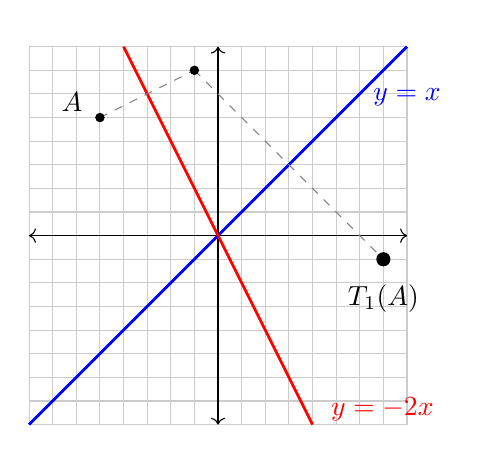
\begin{tikzpicture}[scale=.3]
\draw[thin,gray!40] (-8,-8) grid (8,8);
  \draw[<->] (-8,0)--(8,0);
  \draw[<->] (0,-8)--(0,8);
  \draw[line width=1pt,blue](-8,-8)--(8,8)node[below=4mm]{$y=x$} ;
  \draw[line width=1pt,red](-4,8)--(4,-8)node[above=2mm, right=1mm]{$y=-2x$};
 
  \draw[gray, dashed] (-5,5)--(-1,7);
  \draw[gray, dashed] (-1,7)--(7,-1);
  \fill[] (-5,5)node[above=2mm, left=1mm]{$A$} circle (0.2cm);
  \fill[] (-1,7)node[above=3mm]{} circle (0.2cm);
  \fill[] (7,-1)node[below=2mm]{$T_1(A)$} circle (0.3cm);
  \end{tikzpicture}
  \quad\quad
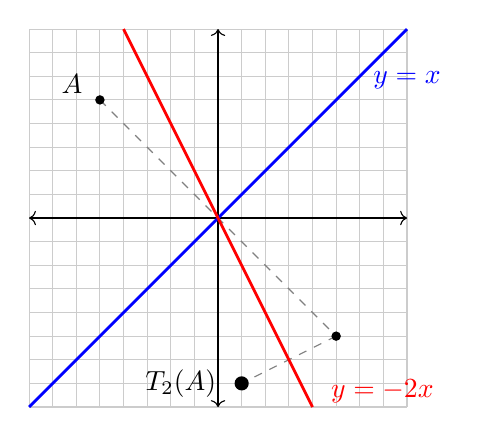
\begin{tikzpicture}[scale=.3]
 
\draw[thin,gray!40] (-8,-8) grid (8,8);
  \draw[<->] (-8,0)--(8,0);
  \draw[<->] (0,-8)--(0,8);
\draw[gray, dashed] (-5,5)--(5,-5);
  \draw[gray, dashed] (5,-5)--(1,-7);
  \fill[] (-5,5)node[above=2mm, left=1mm]{$A$} circle (0.2cm);
  \fill[] (5,-5)node[above=3mm]{} circle (0.2cm);
  \fill[] (1,-7)node[left=2mm]{$T_2(A)$} circle (0.3cm);
  the transformation induced by
  \draw[line width=1pt,blue](-8,-8)--(8,8)node[below=4mm]{$y=x$} ;
  \draw[line width=1pt,red](-4,8)--(4,-8)node[above=2mm, right=1mm]{$y=-2x$} ;
 \end{tikzpicture}
\end{center}
%\caption{A graphical illustration of non-commutativity of matrix multiplication.}
%  \label{fig:reflectioncomp} 
%\end{figure}

Since $T_1\neq T_2$, we conclude that $M_{y=x}M_{y=-2x}\neq M_{y=-2x}M_{y=x}$.

\end{initprob}

\begin{example}\label{ex:rotationscommute}
Some pairs of matrices do commute.  For example, geometry makes it is easy to see that two rotation matrices commute.
\end{example}




 
\subsection*{Inverse of a Linear Transformation}
Recall that two linear transformations are inverses of each other if their composition is the identity transformation.
If a linear transformation $T$ induced by the matrix $M$ is invertible, then $T^{-1}$ is induced by $M^{-1}$.  

Geometry can help find the inverse of certain matrices.  For example, we can easily see that the inverse of the rotation transformation $R_{\theta}:\RR^2\rightarrow \RR^2$ with standard matrix $M_{\theta}$ has the inverse $R_{360^{\circ}-\theta}:\RR^2\rightarrow \RR^2$ with standard matrix $M_{360^{\circ}-\theta}$.

\section*{Practice Problems}
\begin{problem}\label{prob:k0}
Consider matrices $M_v$ and $M_h$ in (\ref{vscale}) and (\ref{hscale}).  
\begin{enumerate}
\item
If we were to allow $k$ to be zero, what would the resulting transformations accomplish?  
\item In what way would the resulting matrices be fundamentally different from matrices $M_v$ and $M_h$ $(k\neq 0)$?  
\item Do $M_v$ and $M_h$ $(k\neq 0)$ have inverses?  What about $M_v$ and $M_h$ $(k= 0)$?  
\item What would happen if we allowed $k$ to be negative?
\end{enumerate}
\end{problem}

\begin{problem} Find the standard matrix $M$ of a linear transformation that would double the length of a photo horizontally, and triple the height of the photo.
$$M=\begin{bmatrix}\answer{2} & \answer{0}\\\answer{0} & \answer{3}\end{bmatrix}$$
\end{problem}

\begin{problem}
(Sheared Sheep) Find the standard matrix of the linear transformation shown in the figure. %\ref{fig:shearedsheep}.

%\begin{figure}[h]
\begin{center}
   
		\begin{tikzpicture}[scale=2]
\node[inner sep=0pt, anchor=base] (gulls) at (8.75mm,0)
  {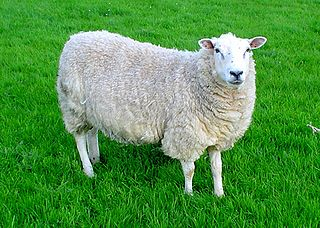
\includegraphics[width=35mm]{sheep.jpg}};
  \draw[<->] (-0.25,0)--(2,0);
  \draw[<->] (0,-0.25)--(0,1.8);
       \end{tikzpicture}
  \quad
\begin{tikzpicture}[scale=2]
 
 \node[inner sep=0pt, anchor=base]  (stretchedgulls) at (12.35mm,0)
  {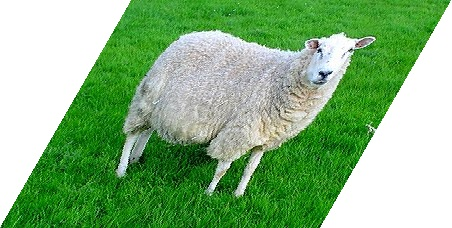
\includegraphics[width=49.4mm]{shearedsheep.jpg}};
  
 \draw (22.3mm,0)node[above=6mm, right=0mm]{$60^{\circ}$} arc (0:60:0.5) ;

\draw[<->] (-0.25,0)--(3,0);
  \draw[<->] (0,-0.25)--(0,1.8);
    
 \end{tikzpicture}
\end{center}
%\caption{Fill in the blank:  A sheep and a \rule{2cm}{0.5pt} sheep.}
%  \label{fig:shearedsheep} 
%\end{figure}
\end{problem}

\begin{problem}\label{prob:linestolines}
In the beginning of this module we claimed that linear transformations leave the origin fixed and map lines to lines.  Prove this claim.
\end{problem}

\begin{problem}\label{prob:translation_does_not_work}

Suppose a 1 by 1 photo of a chipmunk was shifted as shown in the figure. %\ref{fig:translation_does_not_work}.
%\begin{figure}[h]
\begin{center}   
		\begin{tikzpicture}[scale=2]
\node[inner sep=0pt, anchor=base] (gulls) at (6.25mm,0)
  {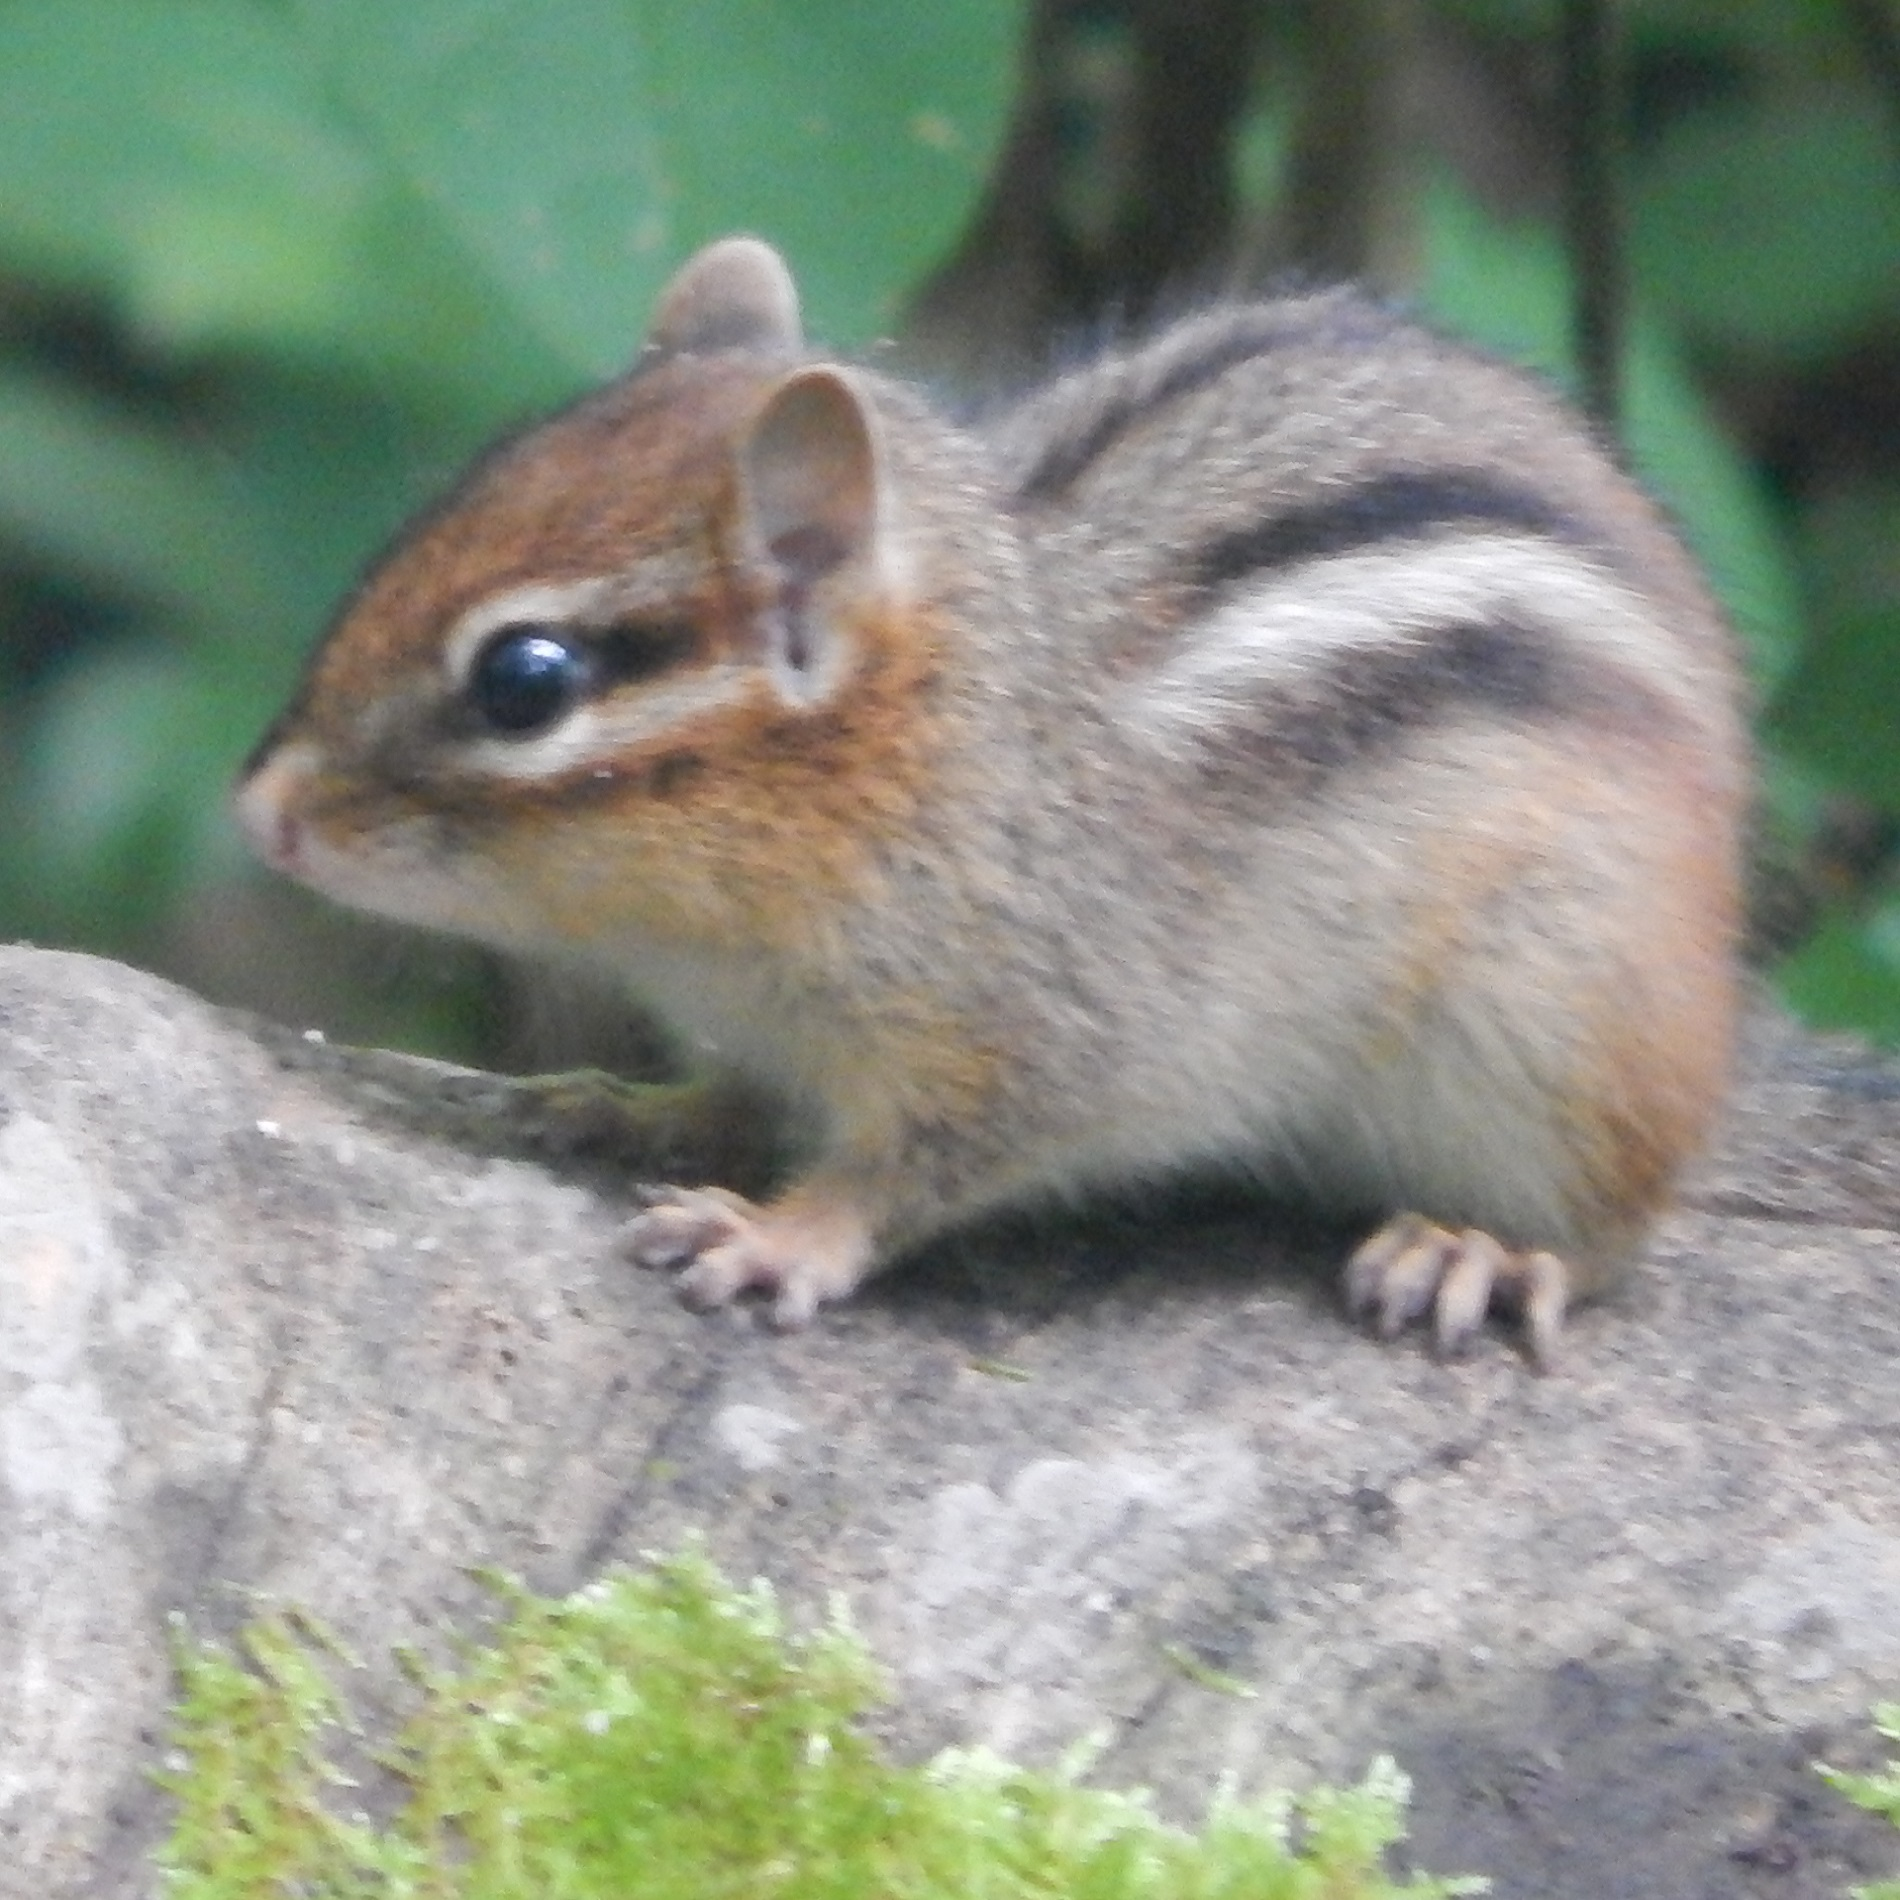
\includegraphics[width=25mm]{chipmunk.jpg}};
  \draw[<->] (-0.5,0)--(2,0);
  \draw[<->] (0,-0.5)--(0,2);
  \draw[->,red, line width=1mm, -stealth] (0mm,0mm)--(12.5mm,0mm)node[below right]{$(1, 0)$};
  \draw[->,blue, line width=1mm, -stealth] (0mm,0mm)--(0mm,12.5mm)node[above left]{$(0, 1)$};
       \end{tikzpicture}
  \quad\quad
   \begin{tikzpicture}[scale=2]
 \node[inner sep=0pt, anchor=base]  (stretchedgulls) at (11.25mm,5mm)
  {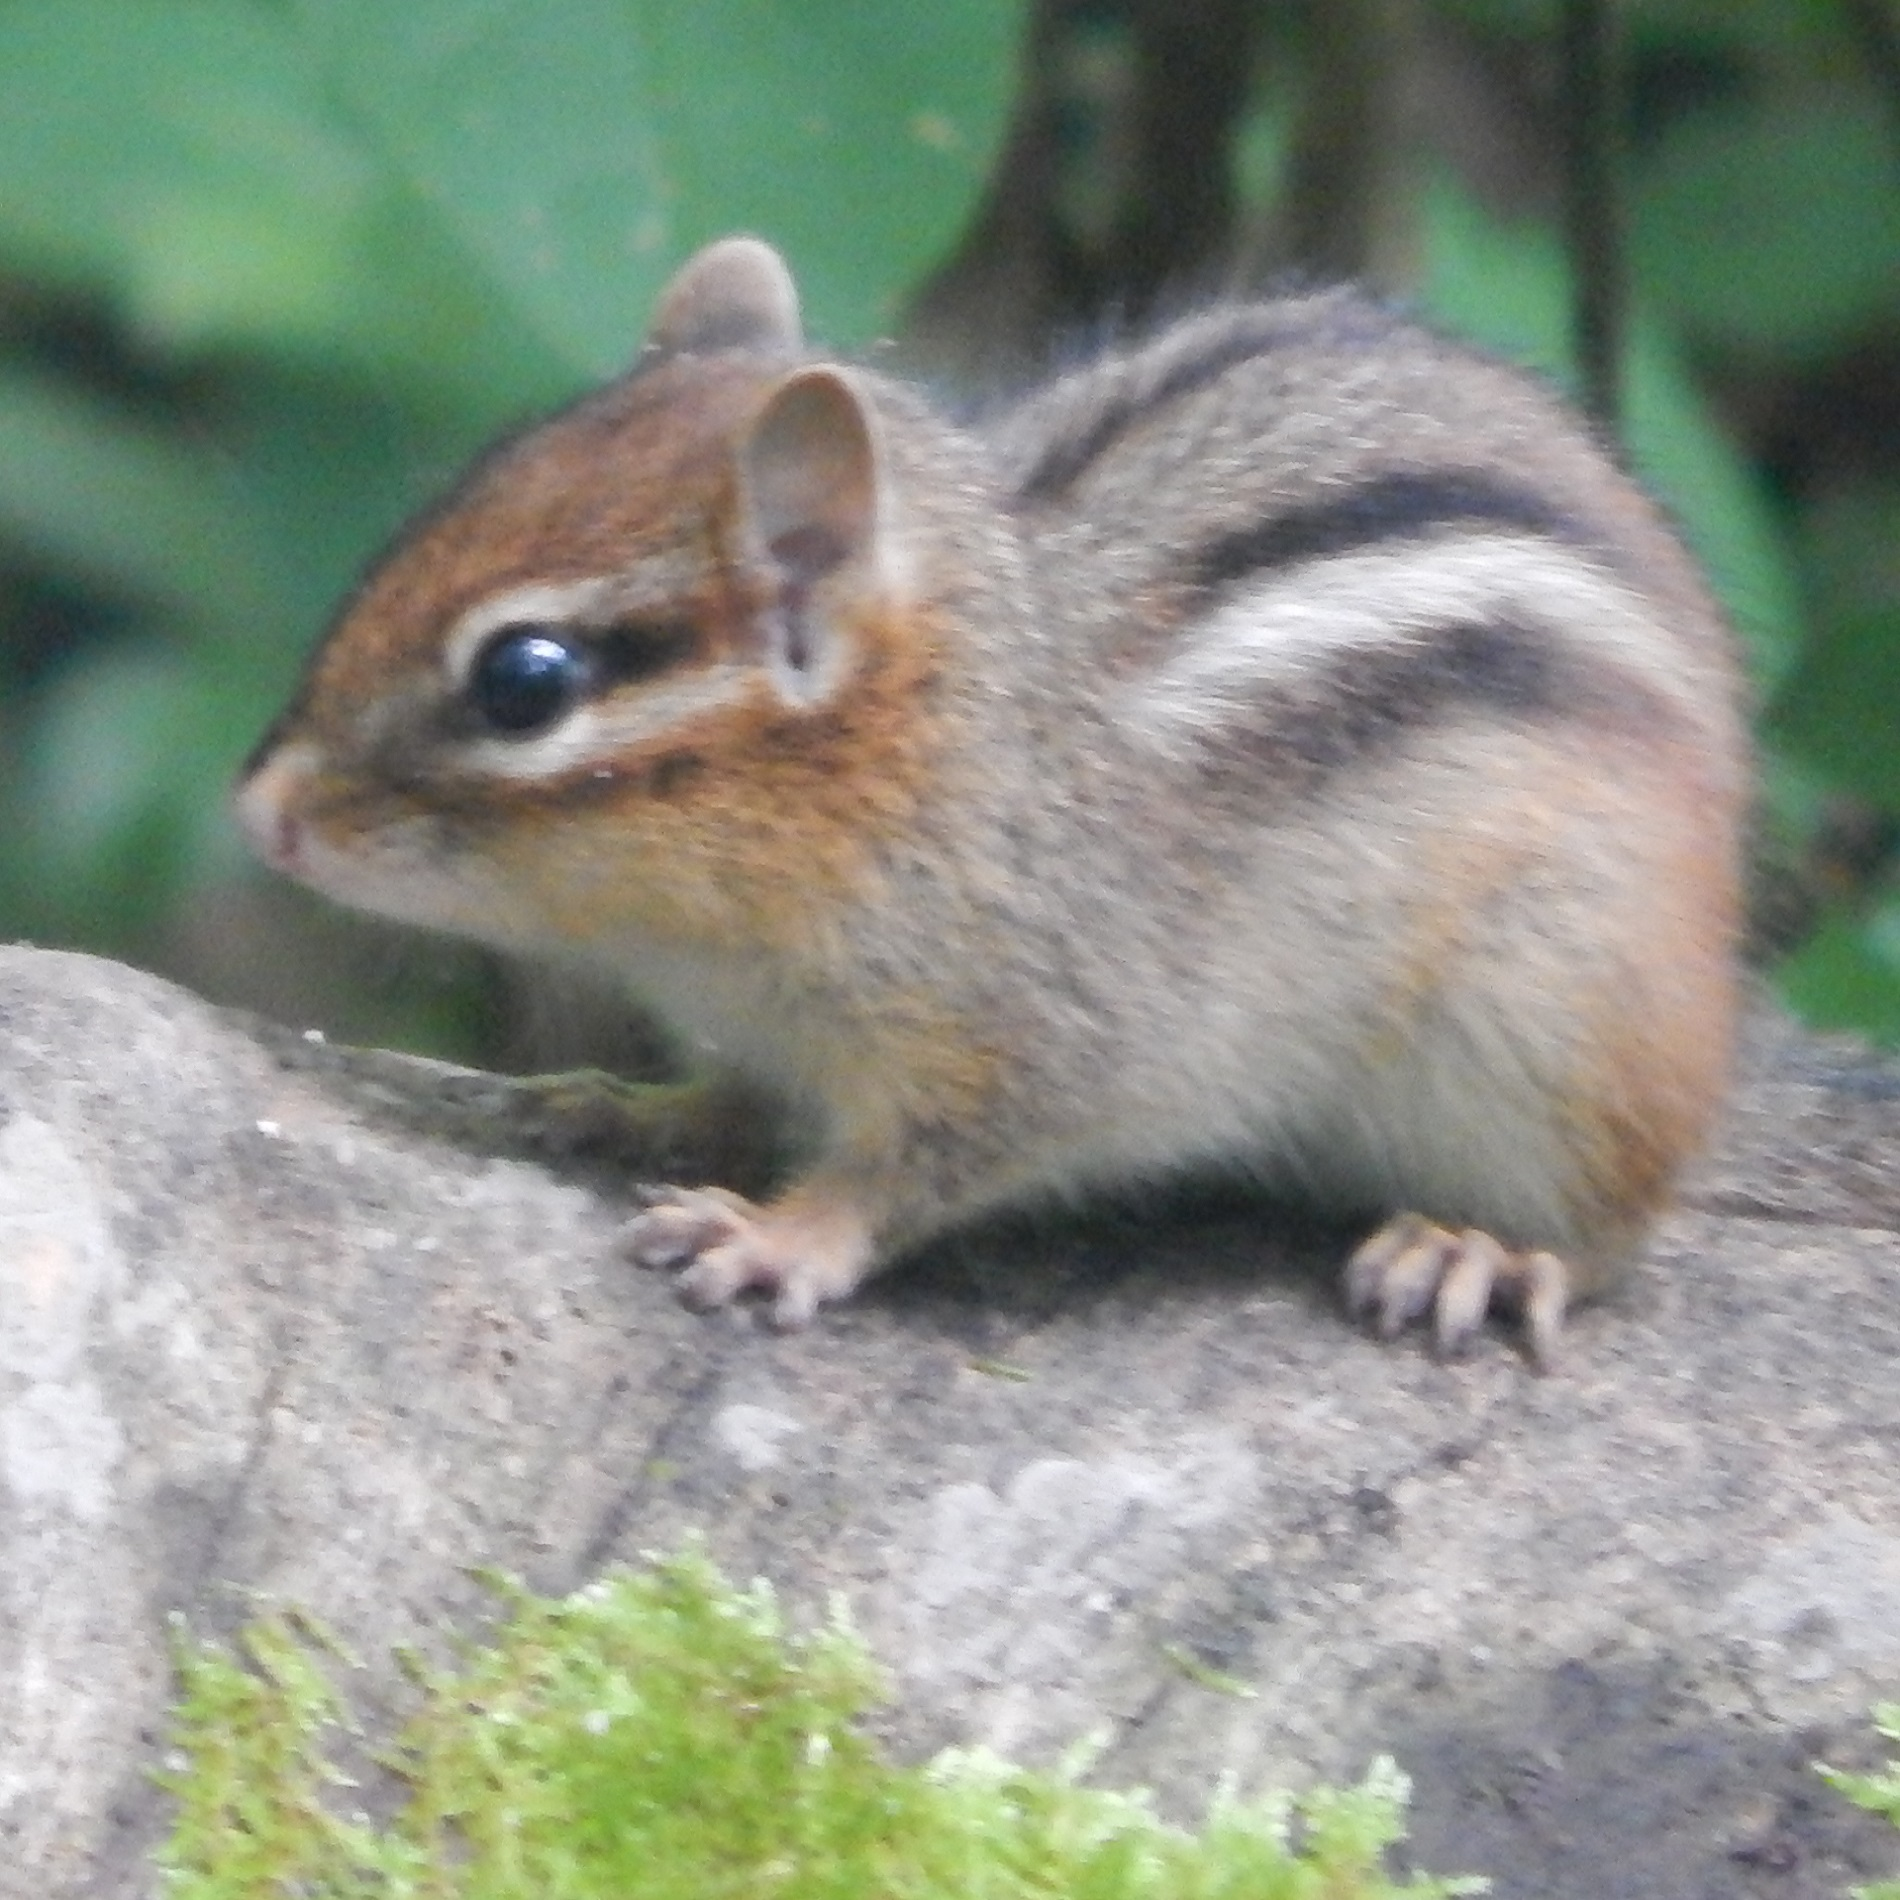
\includegraphics[width=25mm]{chipmunk.jpg}};
\draw[<->] (-0.5,0)--(2,0);
  \draw[<->] (0,-0.5)--(0,2);
  \draw[->,red, line width=1mm, -stealth] (0mm,0mm)--(17.5mm,5mm)node[below right]{$(1.4, 0.4)$};
  \draw[->,blue, line width=1mm, -stealth] (0mm,0mm)--(5mm,17.5mm)node[above right]{$(0.4, 1.4)$};
    \end{tikzpicture}
\end{center}
%\caption{The chipmunk photo was shifted 0.4 units to the right and 0.4 units up.}
 % \label{fig:translation_does_not_work}
%\end{figure}

Suppose we tried to construct a standard matrix $M$ for this transformation by making the images of $\vec{i}$ and $\vec{j}$ the columns of $M$.  We would obtain
$$M=\begin{bmatrix}1.4 & 0.4\\0.4 & 1.4\end{bmatrix}$$
Does this matrix describe the transformation?  If so, prove it.  If not, explain why not.
\end{problem}

\begin{problem}
A transformation $T:\RR^2\rightarrow \RR^2$ that shifts all points in the plane horizontally or vertically by a fixed amount is called a \dfn{translation}.  Is $T$ a linear transformation?  Prove your claim.
\end{problem}

\begin{problem} A reflection about the line $y=mx$ followed by another reflection about the same line, amounts to the identity transformation.  Prove this using matrix multiplication.
\end{problem}

\begin{problem}
Verify Equation (\ref{eq:imageofj}).
\end{problem}

\begin{problem}\label{prob:fixedpoint}
Prove that every point along the line $y=\frac{3}{5}x$ in Example \ref{ex:reflectedduck} is a fixed point.
\end{problem}

\begin{problem}
The figure below shows a sequence of two linear transformations that accomplishes a reflection about the line $y=\frac{3}{5}x$.  The first transformation is a reflection of the plane about the $x$-axis.  The second transformation is a rotation of the plane about the origin.  Find the standard matrices for the two transformations and verify that their product (in the correct order) is the reflection matrix of Example \ref{ex:reflectedduck}.
\end{problem}



%\begin{figure}[h]
\begin{center}
     
		\begin{tikzpicture}[scale=2]
\node[inner sep=0pt, anchor=base] (gulls) at (6.25mm,0)
  {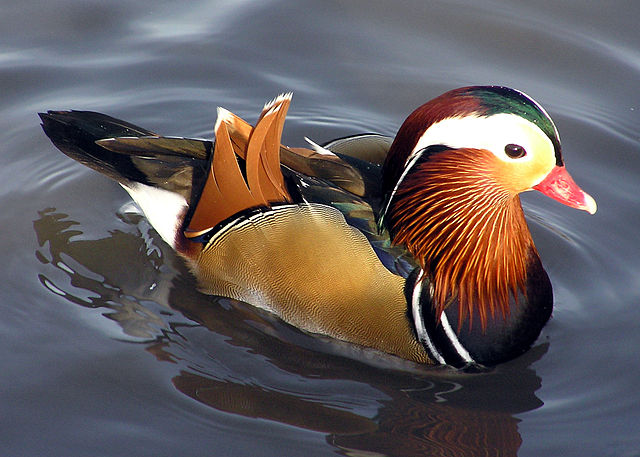
\includegraphics[width=25mm]{duck.jpg}};
  \draw[<->] (-0.5,0)--(2,0);
  \draw[<->] (0,-0.5)--(0,1.5);
  \draw[red,thick] (0,0)--(2,1.2)node[above=2mm, left=1mm]{$y=\frac{3}{5}x$};
       \end{tikzpicture}
  
    
       
		\begin{tikzpicture}[scale=2]
\node[inner sep=0pt, anchor=base] (gulls) at (6.25mm,-8.9mm)
  {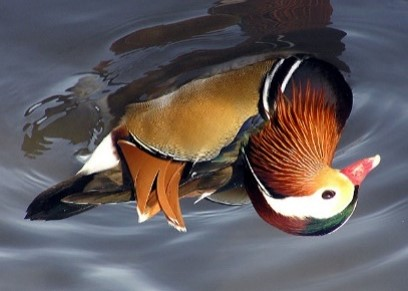
\includegraphics[width=25mm]{upsidedownduck.jpg}};
  \draw[<->] (-0.5,0)--(2,0);
  \draw[<->] (0,-1.5)--(0,1.5);
  \draw[red,thick] (0,0)--(2,1.2)node[above=2mm, left=1mm]{$y=\frac{3}{5}x$};
  \draw[dashed] (0,0)--(0.8,1.5)node[above=2mm, left=1mm]{};
       \end{tikzpicture}
   
    
   
\begin{tikzpicture}[scale=2]
 \node[inner sep=0pt, anchor=base]  (stretchedgulls) at (6.875mm,-4.2mm)
  {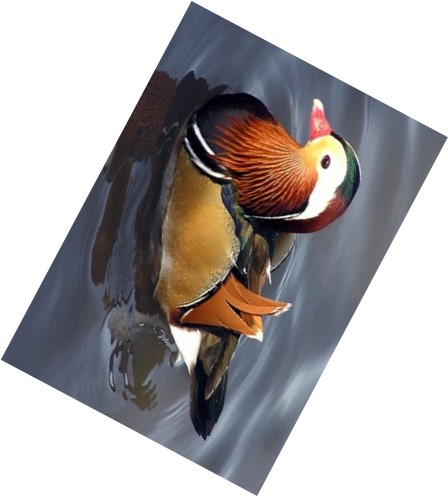
\includegraphics[width=27.5mm]{reflectedduck.jpg}};
  
  
\draw[red,thick] (0,0)--(2,1.2)node[above=2mm, left=1mm]{$y=\frac{3}{5}x$};
\draw[<->] (-0.5,0)--(2,0);
  \draw[<->] (0,-0.5)--(0,1.5);
   \draw[dashed] (0,0)--(0.8,1.5)node[above=2mm, left=1mm]{}; 
 \end{tikzpicture}
\end{center}
%\caption{The photo was first reflected about the $x$-axis, then rotated about the origin.}
%  \label{fig:duckcomp}
%\end{figure}
 


%\section*{Photo Credits}
%The following images are courtesy of \href{https://commons.wikimedia.org/wiki/Main_Page}
%{Wikimedia Commons}
%\vskip 10pt
%\noindent Adrian Pingstone (Figures \ref{fig:reflect}, \ref{fig:duckcomp}), {\it A male Mandarin Duck at Slimbridge Wildfowl and Wetlands Centre, Gloucestershire, England.} Public Domain
%\vskip 10pt
%\noindent Ansgar Koreng (Figure \ref{fig:building}), {\it Facade of ARD-Hauptstadtstudio in Berlin-Mitte.} CC-BY 4.0
%\vskip 10pt
%\noindent Christoph Braun (Figure \ref{fig:rotation}), {\it Reflection of St. Michaelis Church in a window of St. Ansgar in Hamburg, Germany.} Public Domain.
%\vskip 10pt
%\noindent Daniel Gammert (Figure \ref{fig:vstretch}), {\it Red-billed Gulls Chroicocephalus novaehollandiae scopulinus. Brighton Beach, New Zealand.} Public Domain
%\vskip 10pt
%\noindent I, Tony Wills (Figure \ref{fig:vshear}), {\it Red billed gull in Wellington Harbour, Wellington, New Zealand.}  CC-BY
%\vskip 10pt
%\noindent Jackhynes (Figure \ref{fig:sheep}), {\it Lleyn sheep taken with a Sony Digital Camera at 3.2 megapixels in Devon, UK.} Public Domain
%\vskip 10pt

%\noindent Thomas Bresson from Belfort, France (Figure \ref{fig:butterfly}), {\it Old World Swallowtail.} CC-BY




\end{document} 